% vi: tw=0 nowrap
\documentclass[a4paper,landscape,11pt]{article}
\usepackage{graphicx}
\usepackage{amsmath}
\usepackage{amssymb}
\usepackage{caption}
\usepackage{tabularx}
\usepackage{float}
\usepackage{booktabs}
\usepackage[margin=2.5cm]{geometry}

\newcommand{\set}[2]{$#1 \leftarrow #2$}
\newcommand{\incr}[1]{\set{#1}{#1 + 1}}
\newcommand{\decr}[1]{\set{#1}{#1 - 1}}
\newcommand{\rlink}[1]{\texttt{RLINK}(#1)}
\newcommand{\llink}[1]{\texttt{LLINK}(#1)}
\newcommand{\topp}[1]{\texttt{TOP}(#1)}
\newcommand{\ulink}[1]{\texttt{ULINK}(#1)}
\newcommand{\dlink}[1]{\texttt{DLINK}(#1)}
\newcommand{\len}[1]{\texttt{LEN}(#1)}

\title{The Art of Computer Programming---Exercises}
\author{Andreas Wachowski}
\date{}
\begin{document}

\maketitle

\thispagestyle{empty}
\tableofcontents
\listoffigures
\listoftables
\newpage
\pagenumbering{arabic}

\section{Vol. 4B Ex. 11 p. 125, 2025-05-01}

\begin{figure}[H]
	\centering

	\begin{minipage}[t]{0.48\linewidth}
		\centering
		\captionof{table}{Initial memory layout}
		\begin{tabular}{c c c c c c c c c}
			\hline
			$i$:                 & 0   & 1  & 2    & 3    & 4  & 5  & 6    & 7    \\
			$\texttt{NAME}(i)$:  & --- & a  & b    & c    & d  & e  & f    & g    \\
			$\texttt{LLINK}(i)$: & 7   & 0  & 1    & 2    & 3  & 4  & 5    & 6    \\
			$\texttt{RLINK}(i)$: & 1   & 2  & 3    & 4    & 5  & 6  & 7    & 0    \\
			\hline
			$x$:                 & 0   & 1  & 2    & 3    & 4  & 5  & 6    & 7    \\
			$\texttt{LEN}(x)$:   & --- & 2  & 2    & 2    & 3  & 2  & 2    & 3    \\
			$\texttt{ULINK}(x)$: & --- & 20 & 24   & 17   & 27 & 28 & 22   & 29   \\
			$\texttt{DLINK}(x)$: & --- & 12 & 16   & 9    & 13 & 10 & 18   & 14   \\
			\hline
			$x$:                 & 8   & 9  & 10   & 11   & 12 & 13 & 14   & 15   \\
			$\texttt{TOP}(x)$:   & 0   & 3  & 5    & $-1$ & 1  & 4  & 7    & $-2$ \\
			$\texttt{ULINK}(x)$: & --- & 3  & 5    & 9    & 1  & 4  & 7    & 12   \\
			$\texttt{DLINK}(x)$: & 10  & 17 & 28   & 14   & 20 & 21 & 25   & 18   \\
			\hline
			$x$:                 & 16  & 17 & 18   & 19   & 20 & 21 & 22   & 23   \\
			$\texttt{TOP}(x)$:   & 2   & 3  & 6    & $-3$ & 1  & 4  & 6    & $-4$ \\
			$\texttt{ULINK}(x)$: & 2   & 9  & 6    & 16   & 12 & 13 & 18   & 20   \\
			$\texttt{DLINK}(x)$: & 24  & 3  & 22   & 22   & 1  & 27 & 6    & 25   \\
			\hline
			$x$:                 & 24  & 25 & 26   & 27   & 28 & 29 & 30   &      \\
			$\texttt{TOP}(x)$:   & 2   & 7  & $-5$ & 4    & 5  & 7  & $-6$ &      \\
			$\texttt{ULINK}(x)$: & 16  & 14 & 24   & 21   & 10 & 25 & 27   &      \\
			$\texttt{DLINK}(x)$: & 2   & 29 & 29   & 4    & 5  & 7  & ---  &      \\
		\end{tabular}
		\label{tab:initial_memory_layout}
	\end{minipage}
	\hfill
	\begin{minipage}[t]{0.48\linewidth}
		\centering
		\caption{Initial data structure}
		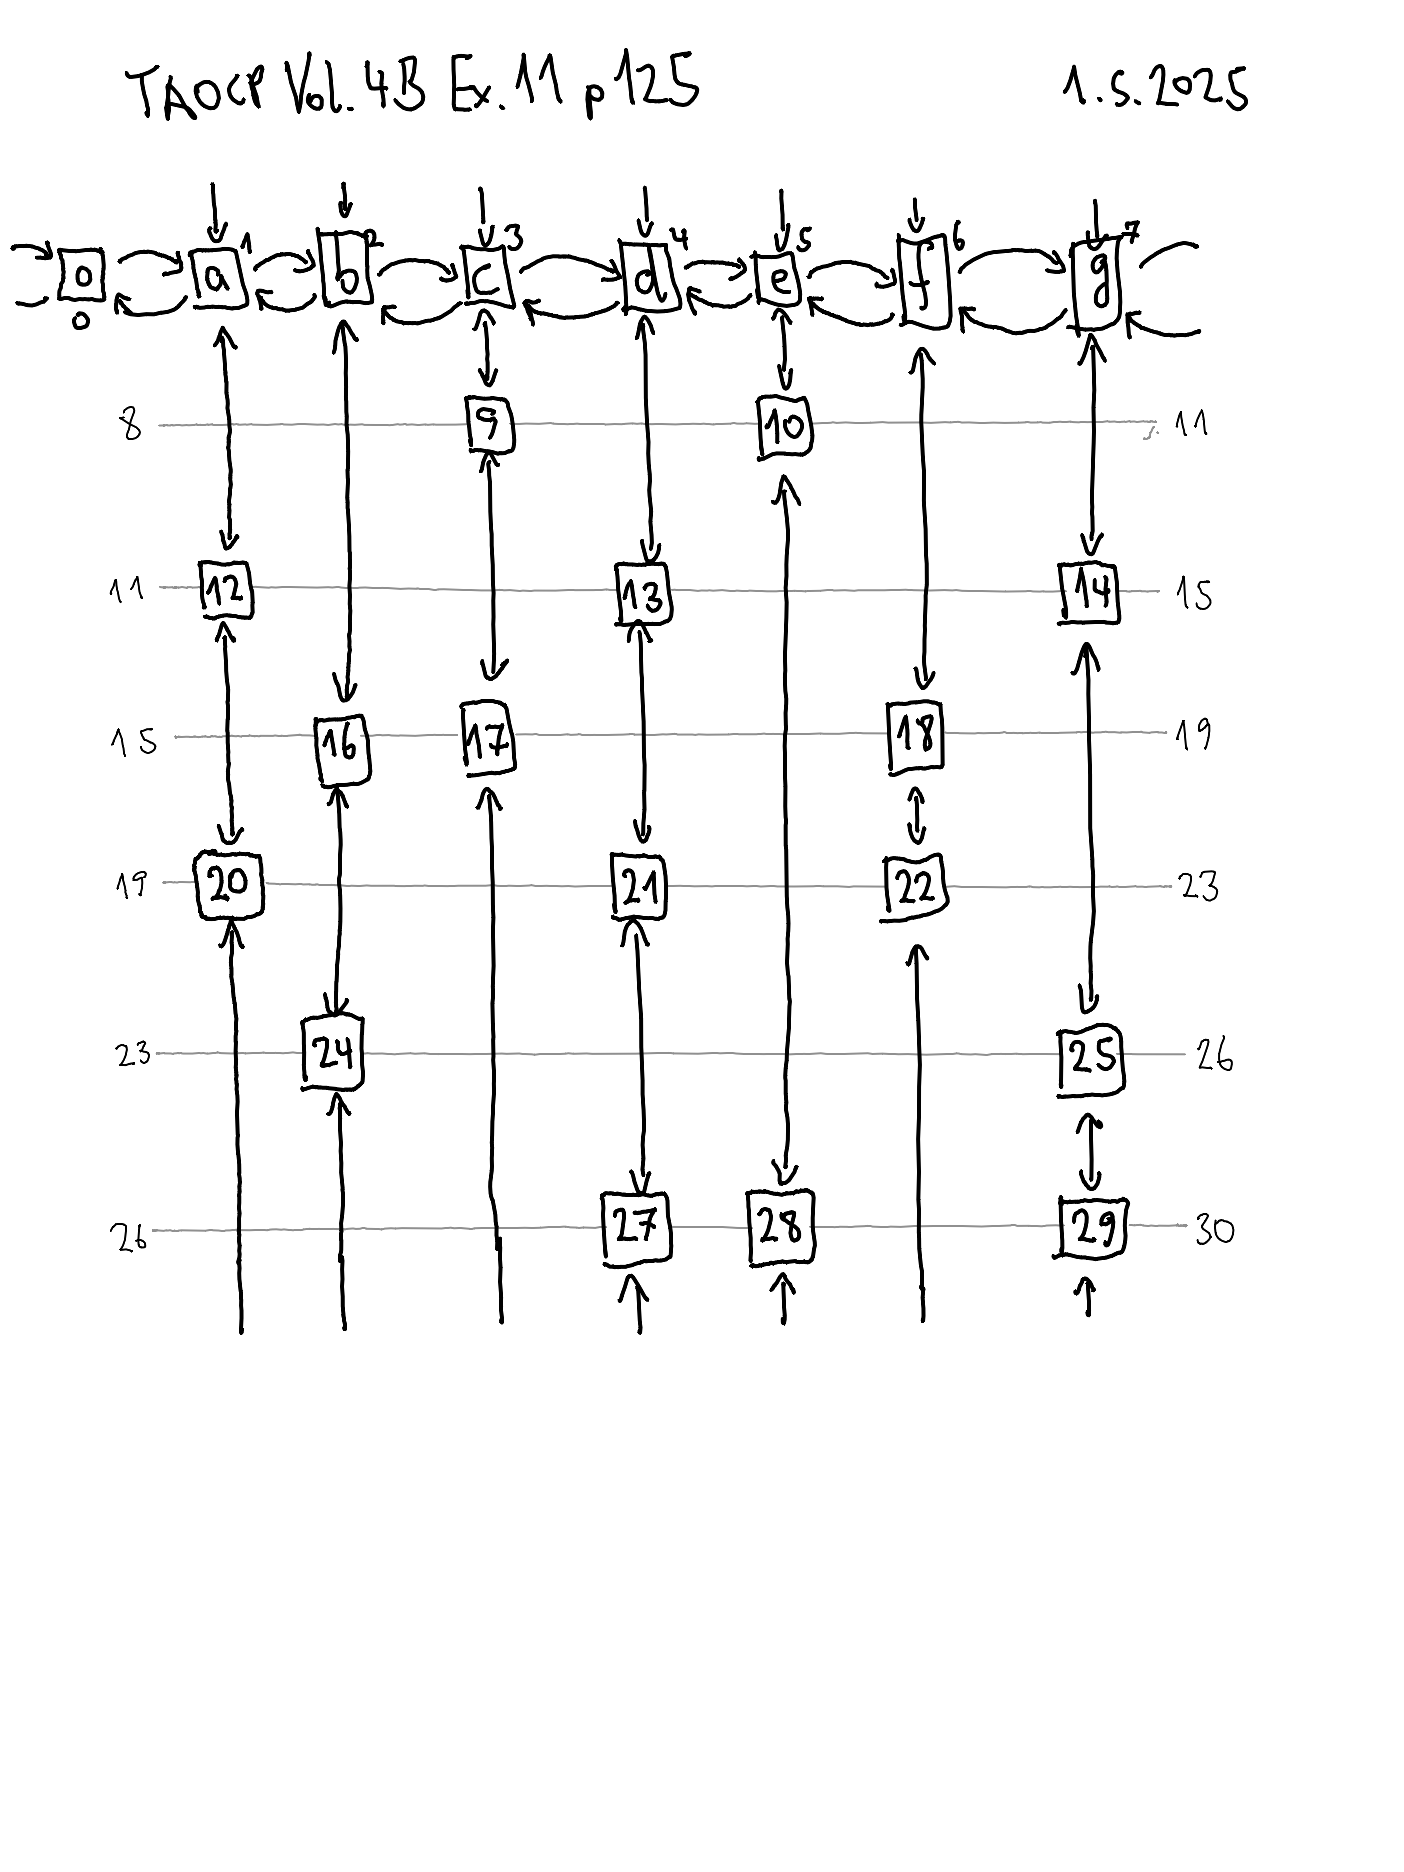
\includegraphics[width=\linewidth]{vol4b_ex11_p125_1.png}
		\label{fig:initial_data_structure}
	\end{minipage}
\end{figure}

\noindent
\begin{tabularx}{\textwidth}{c c c l c c c X}
	\toprule
	\textbf{Step} & $i$ & $l$ & $x_0x_1\ldots x_{l-1}$ & \rlink{0}~$ = 0$ & $x_l = i$ & $p \ne x_l$ & \textbf{Notes / Action}                                                                                 \\
	\midrule
	\textbf{X1.}  &     & 0   &                        &                  &           &             & [Initialize.] \set{N}{7}, \set{Z}{30}, \set{l}{0}                                                       \\
	\textbf{X2.}  &     &     &                        & false            &           &             & [Enter level $l$.] If \rlink{0}~$= 0$ visit solution specified in $x_0x_1\ldots x_{l-1}$ and go to X8.  \\
	\textbf{X3.}  & 1   &     &                        &                  &           &             & [Choose $i$.] by MRV heuristic $(\min\{\texttt{LEN}\} = 2)$ from $i_1i_2\ldots i_t = \{1, 2, 3, 5, 6\}$ \\
	\textbf{X4.}  &     &     & 12                     &                  &           &             & [Cover $i$.] Cover item $i$, then set \set{x_l}{\dlink{i}}.                                             \\
	\textbf{X5.}  &     &     &                        &                  & false     &             & [Try $x_l$.]                                                                                            \\
	\bottomrule
\end{tabularx}

\subsection{X4. Cover(1)}
\noindent
\begin{tabularx}{\textwidth}{c c c c c c X}
	\toprule
	\rlink{l} & \llink{r} & $l$ & $r$ & $p$ & $p \ne i$ & \textbf{Notes / Action}                                                            \\
	\midrule
	          &           &     &     & 12  &           & Set \set{p}{\dlink{i}}.                                                            \\
	          &           &     &     &     & true      & While $p \ne i$, hide($p$), then set \set{p}{\dlink{p}}                            \\
	          &           &     &     &     &           & hide(12)                                                                           \\
	          &           &     &     & 20  &           & Set \set{p}{\dlink{p}}                                                             \\
	          &           &     &     &     & true      &                                                                                    \\
	          &           &     &     &     &           & hide(20)                                                                           \\
	          &           &     &     & 1   &           & Set \set{p}{\dlink{p}}                                                             \\
	          &           &     &     &     & false     &                                                                                    \\
	2         & 0         & 0   & 2   &     &           & Set \set{l}{\llink{i}}, \set{r}{\rlink{i}}, \set{\rlink{l}}{r}, \set{\llink{r}}{l} \\
	\bottomrule
\end{tabularx}

\subsubsection{hide(12)}
\begin{tabularx}{\textwidth}{c c c c c c c c c X}
	\toprule
	\dlink{u} & \ulink{d} & \len{x} & $q$ & $x$  & $u$ & $d$ & $q \ne p$ & $x \le 0$ & \textbf{Notes / Action}                                              \\
	          &           &         & 13  &      &     &     & true      &           & Set \set{q}{p+1}, and repeat while $q \ne p$                         \\
	          &           &         &     & 4    & 4   & 21  &           &           & \set{x}{\topp{q}}, \set{u}{\ulink{q}}, \set{d}{\dlink{q}}            \\
	          &           &         &     &      &     &     &           & false     & If $x \le 0$, set \set{q}{u} ($q$ was a spacer); otherwise           \\
	21        & 4         & 2       & 14  &      &     &     &           &           & set \set{\dlink{u}}{d}, \set{\ulink{d}}{u}, \decr{\len{x}}, \incr{q} \\
	          &           &         &     &      &     &     & true      &           & Repeat while $q \ne p$                                               \\
	          &           &         &     & 7    & 7   & 25  &           &           & \set{x}{\topp{q}}, \set{u}{\ulink{q}}, \set{d}{\dlink{q}}            \\
	          &           &         &     &      &     &     &           & false     & If $x \le 0$, set \set{q}{u} ($q$ was a spacer); otherwise           \\
	25        & 7         & 2       & 15  &      &     &     &           &           & set \set{\dlink{u}}{d}, \set{\ulink{d}}{u}, \decr{\len{x}}, \incr{q} \\
	          &           &         &     &      &     &     & true      &           & Repeat while $q \ne p$                                               \\
	          &           &         &     & $-2$ & 12  & 18  &           &           & \set{x}{\topp{q}}, \set{u}{\ulink{q}}, \set{d}{\dlink{q}}            \\
	          &           &         & 12  &      &     &     &           & true      & If $x \le 0$, set \set{q}{u} ($q$ was a spacer);                     \\
	          &           &         &     &      &     &     & false     &           &                                                                      \\
	\bottomrule
\end{tabularx}

\begin{figure}[H]
	\centering
	\captionof{table}{Memory layout after hide(12)}
	\begin{tabular}{c c c c c c c c c }
		\hline
		$i$:                 & 0   & 1          & 2    & 3    & 4           & 5          & 6    & 7           \\
		$\texttt{NAME}(i)$:  & --- & a          & b    & c    & d           & e          & f    & g           \\
		$\texttt{LLINK}(i)$: & 7   & 0          & 1    & 2    & 3           & 4          & 5    & 6           \\
		$\texttt{RLINK}(i)$: & 1   & 2          & 3    & 4    & 5           & 6          & 7    & 0           \\
		\hline
		$x$:                 & 0   & 1          & 2    & 3    & 4           & 5          & 6    & 7           \\
		$\texttt{LEN}(x)$:   & --- & 2          & 2    & 2    & \textbf{2}  & 2          & 2    & \textbf{2}  \\
		$\texttt{ULINK}(x)$: & --- & 20         & 24   & 17   & 27          & 28         & 22   & 29          \\
		$\texttt{DLINK}(x)$: & --- & 12         & 16   & 9    & \textbf{21} & 10         & 18   & \textbf{25} \\
		\hline
		$x$:                 & 8   & 9          & 10   & 11   & 12          & 13         & 14   & 15          \\
		$\texttt{TOP}(x)$:   & 0   & 3          & 5    & $-1$ & 1           & 4          & 7    & $-2$        \\
		$\texttt{ULINK}(x)$: & --- & 3          & 5    & 9    & 1           & 4          & 7    & 12          \\
		$\texttt{DLINK}(x)$: & 10  & 17         & 28   & 14   & 20          & 21         & 25   & 18          \\
		\hline
		$x$:                 & 16  & 17         & 18   & 19   & 20          & 21         & 22   & 23          \\
		$\texttt{TOP}(x)$:   & 2   & 3          & 6    & $-3$ & 1           & 4          & 6    & $-4$        \\
		$\texttt{ULINK}(x)$: & 2   & 9          & 6    & 16   & 12          & \textbf{4} & 18   & 20          \\
		$\texttt{DLINK}(x)$: & 24  & 3          & 22   & 22   & 1           & 27         & 6    & 25          \\
		\hline
		$x$:                 & 24  & 25         & 26   & 27   & 28          & 29         & 30   &             \\
		$\texttt{TOP}(x)$:   & 2   & 7          & $-5$ & 4    & 5           & 7          & $-6$ &             \\
		$\texttt{ULINK}(x)$: & 16  & \textbf{7} & 24   & 21   & 10          & 25         & 27   &             \\
		$\texttt{DLINK}(x)$: & 2   & 29         & 29   & 4    & 5           & 7          & ---  &             \\
	\end{tabular}
\end{figure}

\subsubsection{hide(20)}
\begin{tabularx}{\textwidth}{c c c c c c c c c X}
	\toprule
	\dlink{u} & \ulink{d} & \len{x} & $q$ & $x$  & $u$ & $d$ & $q \ne p$ & $x \le 0$ & \textbf{Notes / Action}                                              \\
	\midrule
	          &           &         & 21  &      &     &     & true      &           & Set \set{q}{p+1}, and repeat while $q \ne p$                         \\
	          &           &         &     & 4    & 4   & 27  &           &           & \set{x}{\topp{q}}, \set{u}{\ulink{q}}, \set{d}{\dlink{q}}            \\
	          &           &         &     &      &     &     &           & false     & If $x \le 0$, set \set{q}{u} ($q$ was a spacer); otherwise           \\
	27        & 4         & 1       & 22  &      &     &     &           &           & set \set{\dlink{u}}{d}, \set{\ulink{d}}{u}, \decr{\len{x}}, \incr{q} \\
	          &           &         &     &      &     &     & true      &           & Repeat while $q \ne p$                                               \\
	          &           &         &     & 6    & 18  & 6   &           &           & \set{x}{\topp{q}}, \set{u}{\ulink{q}}, \set{d}{\dlink{q}}            \\
	          &           &         &     &      &     &     &           & false     & If $x \le 0$, set \set{q}{u} ($q$ was a spacer); otherwise           \\
	6         & 18        & 1       & 23  &      &     &     &           &           & set \set{\dlink{u}}{d}, \set{\ulink{d}}{u}, \decr{\len{x}}, \incr{q} \\
	          &           &         &     &      &     &     & true      &           & Repeat while $q \ne p$                                               \\
	          &           &         &     & $-4$ & 20  & 25  &           &           & \set{x}{\topp{q}}, \set{u}{\ulink{q}}, \set{d}{\dlink{q}}            \\
	          &           &         &     &      &     &     &           & true      & If $x \le 0$,                                                        \\
	          &           &         & 20  &      &     &     &           &           & set \set{q}{u} ($q$ was a spacer);                                   \\
	          &           &         &     &      &     &     & false     &           & Repeat while $q \ne p$                                               \\
	\bottomrule
\end{tabularx}

\begin{figure}[H]
	\centering

	\begin{minipage}[t]{0.48\linewidth}
		\centering
		\captionof{table}{Memory layout after cover(1)}
		\begin{tabular}{c c c c c c c c c}
			\hline
			$i$:                 & 0          & 1  & 2          & 3          & 4           & 5  & 6           & 7    \\
			$\texttt{NAME}(i)$:  & ---        & a  & b          & c          & d           & e  & f           & g    \\
			$\texttt{LLINK}(i)$: & 7          & 0  & \textbf{0} & 2          & 3           & 4  & 5           & 6    \\
			$\texttt{RLINK}(i)$: & \textbf{2} & 2  & 3          & 4          & 5           & 6  & 7           & 0    \\
			\hline
			$x$:                 & 0          & 1  & 2          & 3          & 4           & 5  & 6           & 7    \\
			$\texttt{LEN}(x)$:   & ---        & 2  & 2          & 2          & \textbf{1}  & 2  & \textbf{1}  & 2    \\
			$\texttt{ULINK}(x)$: & ---        & 20 & 24         & 17         & 27          & 28 & \textbf{18} & 29   \\
			$\texttt{DLINK}(x)$: & ---        & 12 & 16         & 9          & \textbf{27} & 10 & 18          & 25   \\
			\hline
			$x$:                 & 8          & 9  & 10         & 11         & 12          & 13 & 14          & 15   \\
			$\texttt{TOP}(x)$:   & 0          & 3  & 5          & $-1$       & 1           & 4  & 7           & $-2$ \\
			$\texttt{ULINK}(x)$: & ---        & 3  & 5          & 9          & 1           & 4  & 7           & 12   \\
			$\texttt{DLINK}(x)$: & 10         & 17 & 28         & 14         & 20          & 21 & 25          & 18   \\
			\hline
			$x$:                 & 16         & 17 & 18         & 19         & 20          & 21 & 22          & 23   \\
			$\texttt{TOP}(x)$:   & 2          & 3  & 6          & $-3$       & 1           & 4  & 6           & $-4$ \\
			$\texttt{ULINK}(x)$: & 2          & 9  & 6          & 16         & 12          & 4  & 18          & 20   \\
			$\texttt{DLINK}(x)$: & 24         & 3  & \textbf{6} & 22         & 1           & 27 & 6           & 25   \\
			\hline
			$x$:                 & 24         & 25 & 26         & 27         & 28          & 29 & 30          &      \\
			$\texttt{TOP}(x)$:   & 2          & 7  & $-5$       & 4          & 5           & 7  & $-6$        &      \\
			$\texttt{ULINK}(x)$: & 16         & 7  & 24         & \textbf{4} & 10          & 25 & 27          &      \\
			$\texttt{DLINK}(x)$: & 2          & 29 & 29         & 4          & 5           & 7  & ---         &      \\
		\end{tabular}
		\label{tab:mem_layout_after_cover_1}
	\end{minipage}
	\hfill
	\begin{minipage}[t]{0.48\linewidth}
		\centering
		\caption{Data structure after cover(1)}
		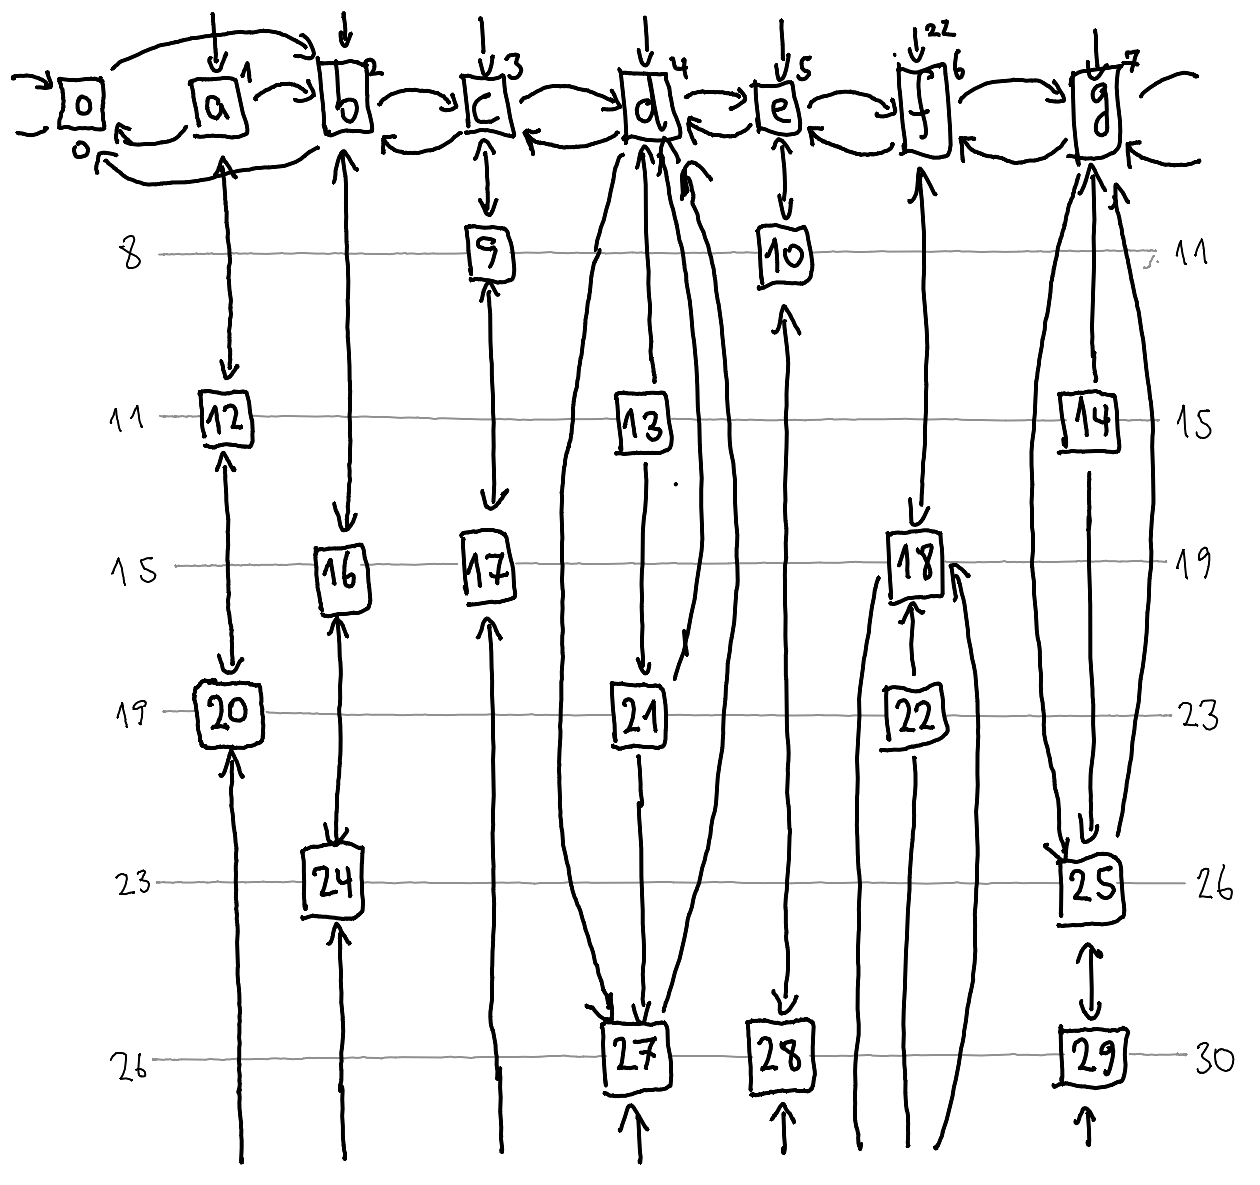
\includegraphics[width=\linewidth]{vol4b_ex11_p125_2.png}
		\label{fig:data_structure_after_cover_1}
	\end{minipage}
\end{figure}

\subsection{X5. Try $x_l = x_0 = 12$}

\begin{tabularx}{\textwidth}{c c c c c c c X}
	\toprule
	$i$ & l   & $x_l = i$ & $p$ & $p \ne x_l$ & $j$ & $j \le 0$ & \textbf{Notes / Action}                                                                         \\
	\midrule
	(1) & (0) & false     & 13  & true        &     &           & If $x_l = i$, go to X7. Otherwise set \set{p}{x_l + 1}, and do the following while $p \ne x_l$. \\
	    &     &           &     &             & 4   &           & Set \set{j}{\topp{p}}                                                                           \\
	    &     &           &     & 14          &     & true      & If $j \le 0$, set \set{p}{\ulink{p}}; otherwise cover($j$) and set \incr{p}.                    \\
	    & 1   &           &     &             &     &           & Set \incr{l} and return to X2.                                                                  \\
	\bottomrule
\end{tabularx}

\subsection{cover($i = 4$)}
\noindent
\begin{tabularx}{\textwidth}{c c c c c c X}
	\toprule
	\rlink{l} & \llink{r} & $l$ & $r$ & $p$ & $p \ne i$ & \textbf{Notes / Action}                                                            \\
	\midrule
	          &           &     &     & 27  &           & Set \set{p}{\dlink{i}}.                                                            \\
	          &           &     &     &     & true      & While $p \ne i$, hide($p$), then set \set{p}{\dlink{p}}                            \\
	          &           &     &     &     &           & hide(27)                                                                           \\

	          &           &     &     & 4   &           & Set \set{p}{\dlink{p}}                                                             \\
	          &           &     &     &     & false     & While $p \ne i$, hide($p$), then set \set{p}{\dlink{p}}                            \\
	5         & 3         & 3   & 5   &     &           & Set \set{l}{\llink{i}}, \set{r}{\rlink{i}}, \set{\rlink{l}}{r}, \set{\llink{r}}{l} \\
	\bottomrule
\end{tabularx}

\subsubsection{hide(27)}
\begin{tabularx}{\textwidth}{c c c c c c c c c X}
	\toprule
	\dlink{u} & \ulink{d} & \len{x} & $q$ & $x$  & $u$ & $d$ & $q \ne p$ & $x \le 0$ & \textbf{Notes / Action}                                              \\
	\midrule
	          &           &         & 28  &      &     &     & true      &           & Set \set{q}{p+1}, and repeat while $q \ne p$                         \\
	          &           &         &     & 5    & 10  & 5   &           &           & \set{x}{\topp{q}}, \set{u}{\ulink{q}}, \set{d}{\dlink{q}}            \\
	          &           &         &     &      &     &     &           & false     & If $x \le 0$, set \set{q}{u} ($q$ was a spacer); otherwise           \\
	5         & 10        & 1       & 29  &      &     &     &           &           & set \set{\dlink{u}}{d}, \set{\ulink{d}}{u}, \decr{\len{x}}, \incr{q} \\
	          &           &         &     &      &     &     & true      &           & Repeat while $q \ne p$                                               \\
	          &           &         &     & 7    & 25  & 7   &           &           & \set{x}{\topp{q}}, \set{u}{\ulink{q}}, \set{d}{\dlink{q}}            \\
	          &           &         &     &      &     &     &           & false     & If $x \le 0$, set \set{q}{u} ($q$ was a spacer); otherwise           \\
	7         & 25        & 1       & 30  &      &     &     &           &           & \set{\dlink{u}}{d}, \set{\ulink{d}}{u}, \decr{\len{x}}, \incr{q}     \\
	          &           &         &     &      &     &     & true      &           & Repeat while $q \ne p$                                               \\
	          &           &         &     & $-6$ & 27  & --- &           &           & \set{x}{\topp{q}}, \set{u}{\ulink{q}}, \set{d}{\dlink{q}}            \\
	          &           &         & 27  &      &     &     &           & true      & If $x \le 0$, set \set{q}{u} ($q$ was a spacer)                      \\
	          &           &         &     &      &     &     & false     &           & Repeat while $q \ne p$                                               \\
	\bottomrule
\end{tabularx}

\begin{figure}[H]
	\centering

	\begin{minipage}[t]{0.48\linewidth}
		\centering
		\captionof{table}{Memory layout after cover(4)}
		\begin{tabular}{c c c c c c c c c}
			\hline
			$i$:                 & 0   & 1          & 2          & 3          & 4  & 5           & 6    & 7           \\
			$\texttt{NAME}(i)$:  & --- & a          & b          & c          & d  & e           & f    & g           \\
			$\texttt{LLINK}(i)$: & 7   & 0          & 0          & 2          & 3  & \textbf{3}  & 5    & 6           \\
			$\texttt{RLINK}(i)$: & 2   & 2          & 3          & \textbf{5} & 5  & 6           & 7    & 0           \\
			\hline
			$x$:                 & 0   & 1          & 2          & 3          & 4  & 5           & 6    & 7           \\
			$\texttt{LEN}(x)$:   & --- & 2          & 2          & 2          & 1  & \textbf{1}  & 1    & \textbf{1}  \\
			$\texttt{ULINK}(x)$: & --- & 20         & 24         & 17         & 27 & \textbf{10} & 18   & \textbf{25} \\
			$\texttt{DLINK}(x)$: & --- & 12         & 16         & 9          & 27 & 10          & 18   & 25          \\
			\hline
			$x$:                 & 8   & 9          & 10         & 11         & 12 & 13          & 14   & 15          \\
			$\texttt{TOP}(x)$:   & 0   & 3          & 5          & $-1$       & 1  & 4           & 7    & $-2$        \\
			$\texttt{ULINK}(x)$: & --- & 3          & 5          & 9          & 1  & 4           & 7    & 12          \\
			$\texttt{DLINK}(x)$: & 10  & 17         & \textbf{5} & 14         & 20 & 21          & 25   & 18          \\
			\hline
			$x$:                 & 16  & 17         & 18         & 19         & 20 & 21          & 22   & 23          \\
			$\texttt{TOP}(x)$:   & 2   & 3          & 6          & $-3$       & 1  & 4           & 6    & $-4$        \\
			$\texttt{ULINK}(x)$: & 2   & 9          & 6          & 16         & 12 & 4           & 18   & 20          \\
			$\texttt{DLINK}(x)$: & 24  & 3          & 6          & 22         & 1  & 27          & 6    & 25          \\
			\hline
			$x$:                 & 24  & 25         & 26         & 27         & 28 & 29          & 30   &             \\
			$\texttt{TOP}(x)$:   & 2   & 7          & $-5$       & 4          & 5  & 7           & $-6$ &             \\
			$\texttt{ULINK}(x)$: & 16  & 7          & 24         & 4          & 10 & 25          & 27   &             \\
			$\texttt{DLINK}(x)$: & 2   & \textbf{7} & 29         & 4          & 5  & 7           & ---  &             \\
		\end{tabular}
		\label{tab:mem_layout_after_cover_4}
	\end{minipage}
	\hfill
	\begin{minipage}[t]{0.48\linewidth}
		\centering
		\caption{Data structure after cover(4)}
		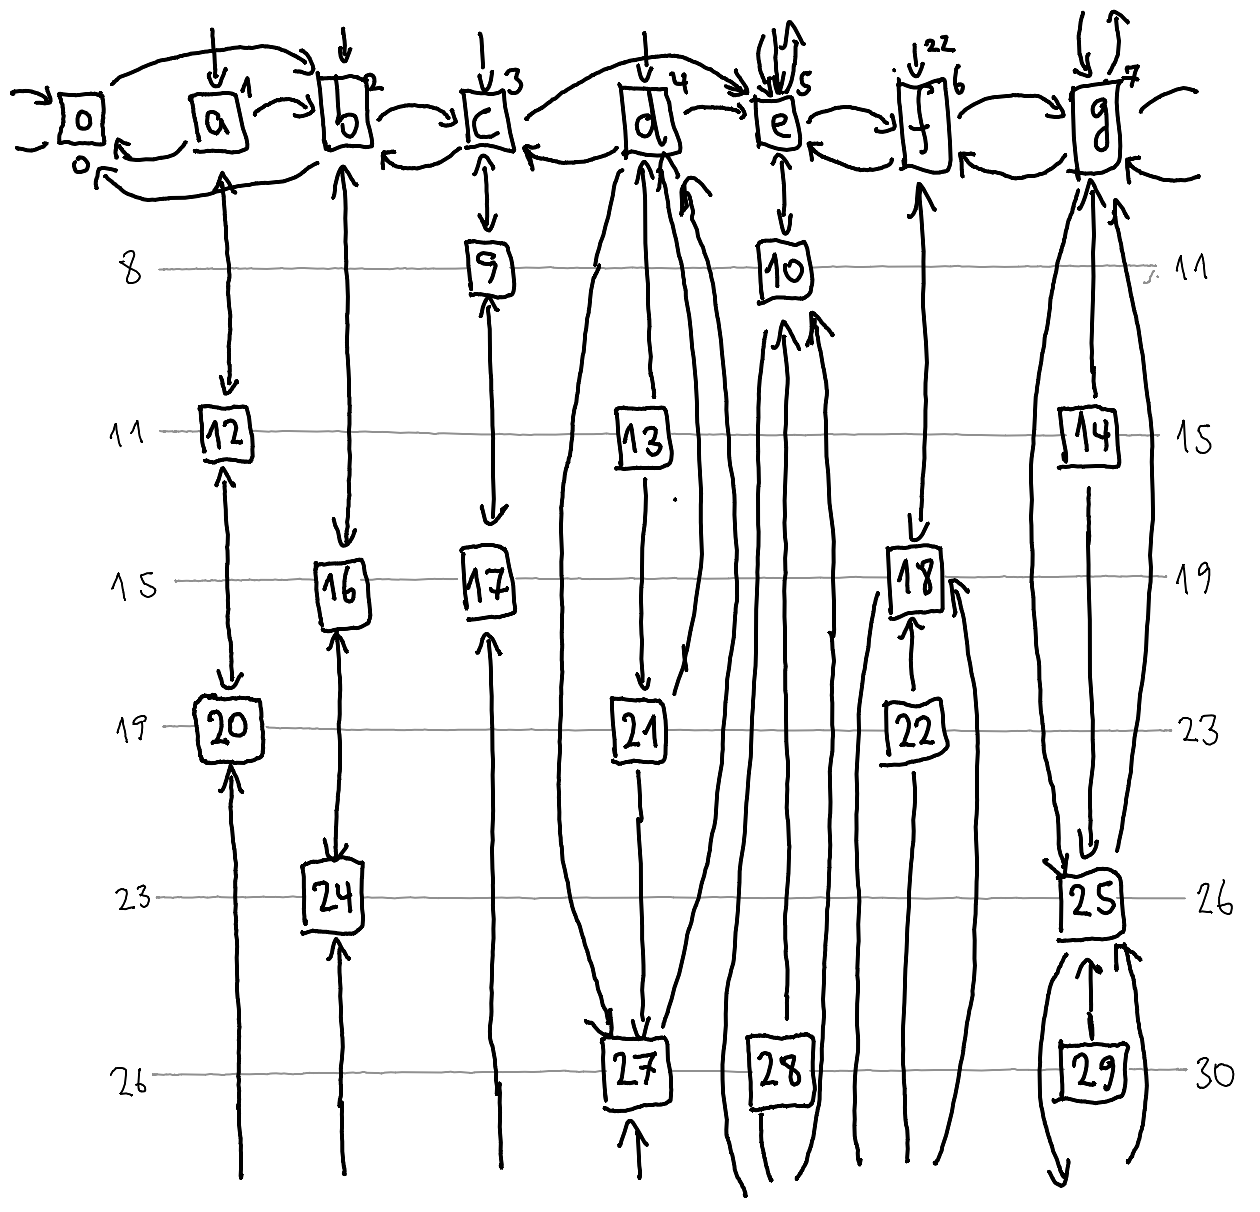
\includegraphics[width=\linewidth]{vol4b_ex11_p125_3.png}
		\label{fig:data_structure_after_cover_4}
	\end{minipage}
\end{figure}


\end{document}
